\section{Integrazione di Kepler per il monitoraggio energetico}

Il monitoraggio dei consumi energetici a livello di container costituisce 
il fondamento del sistema realizzato. A tal fine è stato adottato Kepler 
(Kubernetes-based Efficient Power Level Exporter), uno strumento open 
source sviluppato nell'ambito della CNCF (Cloud Native Computing 
Foundation) che stima il consumo energetico di processi, container e 
pod Kubernetes attraverso l'accesso diretto alle interfacce hardware del 
sistema operativo host~\cite{keplerCNCF2023}.

La scelta di Kepler è motivata principalmente dalla sua granularità di 
misurazione, che opera a livello di singolo container Docker: questa 
corrisponde esattamente all'unità di esecuzione delle funzioni serverless 
in Serverledge. Kepler espone inoltre le proprie metriche nel formato 
standard Prometheus, consentendo un'integrazione diretta con l'ecosistema 
di monitoraggio senza richiedere componenti aggiuntivi per la raccolta 
dei dati.

\subsection{Funzionamento di Kepler}

Kepler opera combinando due meccanismi complementari per associare i 
consumi energetici ai singoli container. Il primo è un programma eBPF 
(Extended Berkeley Packet Filter) integrato nel kernel, che traccia 
l'attività dei processi e li associa ai container tramite il file 
\texttt{/proc/PID/cgroup}, consentendo di correlare il Process ID di 
ciascun processo all'identificatore del container che lo ospita. Il 
secondo è l'interfaccia RAPL (Running Average Power Limit), disponibile 
sui processori Intel e AMD moderni, che permette di leggere i contatori 
energetici cumulativi direttamente dai registri hardware della CPU.

Una volta raccolti i dati di utilization dei processi e di consumo 
energetico del sistema, Kepler applica il \emph{Ratio Power Model} per 
attribuire a ciascun container la propria quota di consumo: la potenza 
dinamica viene distribuita tra i container in proporzione alla loro 
utilization rispetto all'utilization totale del sistema. Il risultato 
viene aggregato a livello di container e reso disponibile tramite 
Prometheus nella metrica \texttt{kepler\_container\_cpu\_joules\_total}, 
un contatore cumulativo espresso in Joule che cresce monotonicamente nel 
tempo per ogni container attivo.

\begin{figure}[ht]
    \centering
    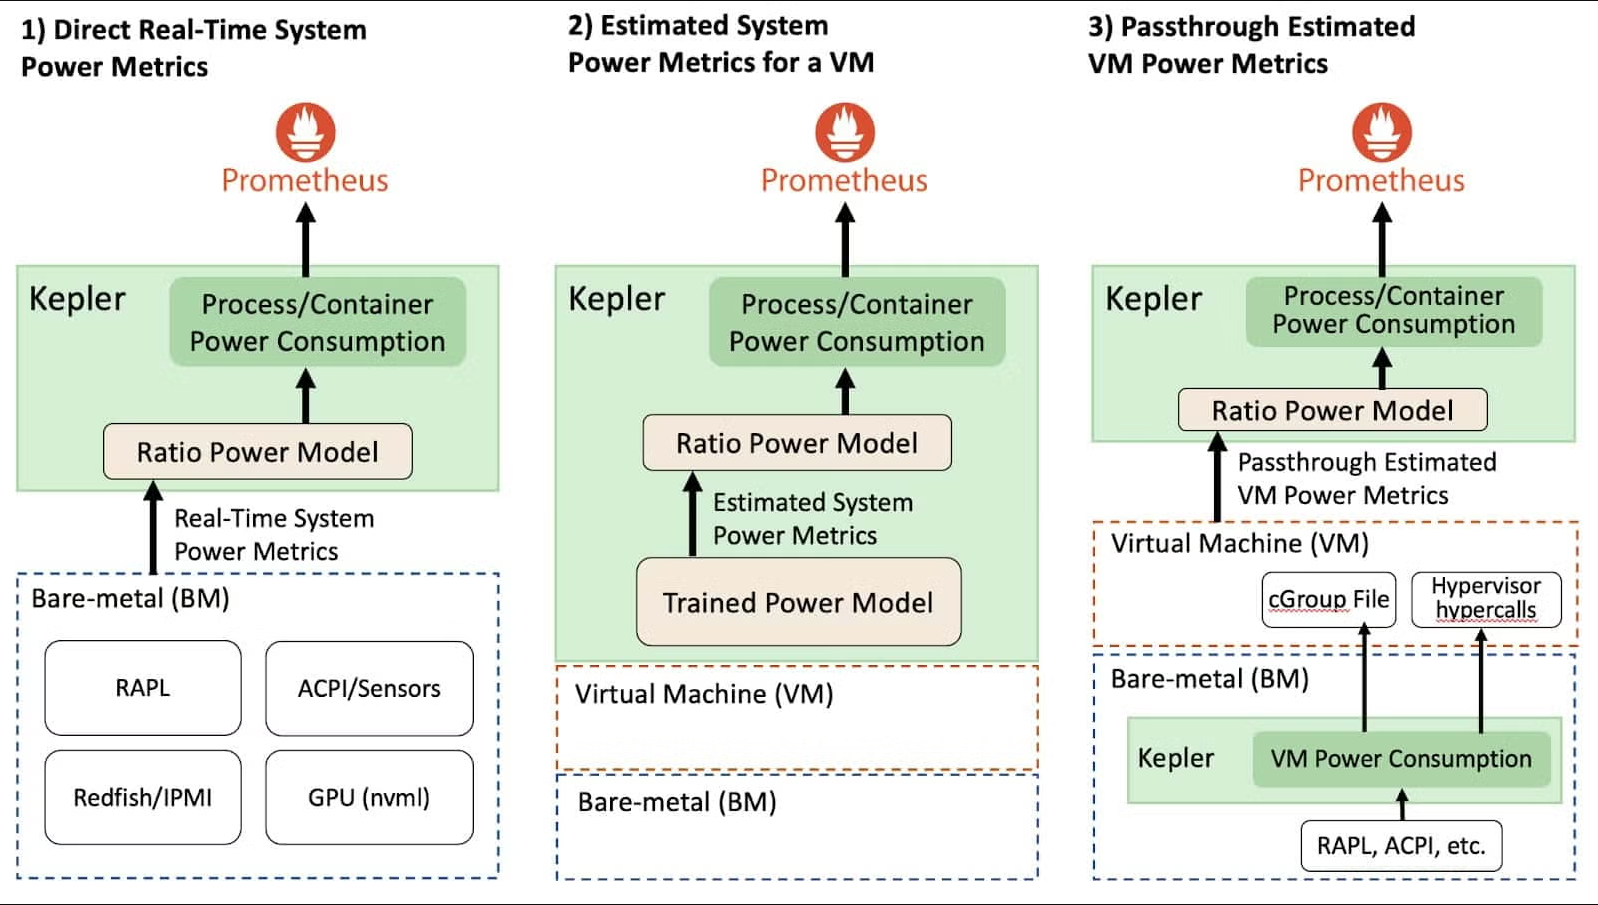
\includegraphics[width=0.85\textwidth]{figures/KeplerArchitecture.jpg}
    \caption{Architettura di Kepler per la raccolta dei consumi energetici 
    in ambienti bare-metal e virtuali. In ambienti bare-metal, Kepler 
    accede direttamente ai contatori hardware tramite RAPL, ottenendo 
    misurazioni real-time senza necessità di modelli predittivi. }
    \label{fig:kepler-arch}
\end{figure}

Come illustrato in Figura~\ref{fig:kepler-arch}, il comportamento di
Kepler varia in base all'ambiente di esecuzione. In ambienti bare-metal,
Kepler accede direttamente ai contatori RAPL, ottenendo misurazioni
energetiche real-time senza ricorrere a modelli predittivi
pre-addestrati. In ambienti virtualizzati, invece, l'assenza di accesso
diretto all'hardware richiede l'uso di modelli di regressione,
introducendo le relative limitazioni di accuratezza.

Per accedere alle interfacce hardware necessarie, Kepler deve essere 
eseguito con privilegi elevati sull'host: richiede accesso a 
\texttt{/sys} e \texttt{/proc} per leggere i contatori RAPL e i cgroup, 
e al socket Docker per identificare i container attivi e associarvi le 
metriche energetiche.

\subsection{Infrastruttura di supporto}

L'avvio dell'infrastruttura di monitoraggio è gestito dallo script 
\texttt{StartMetrics.sh}, che inizializza come container Docker tutti 
i servizi necessari al funzionamento del sistema.  
\begin{figure}[H]
    \centering
    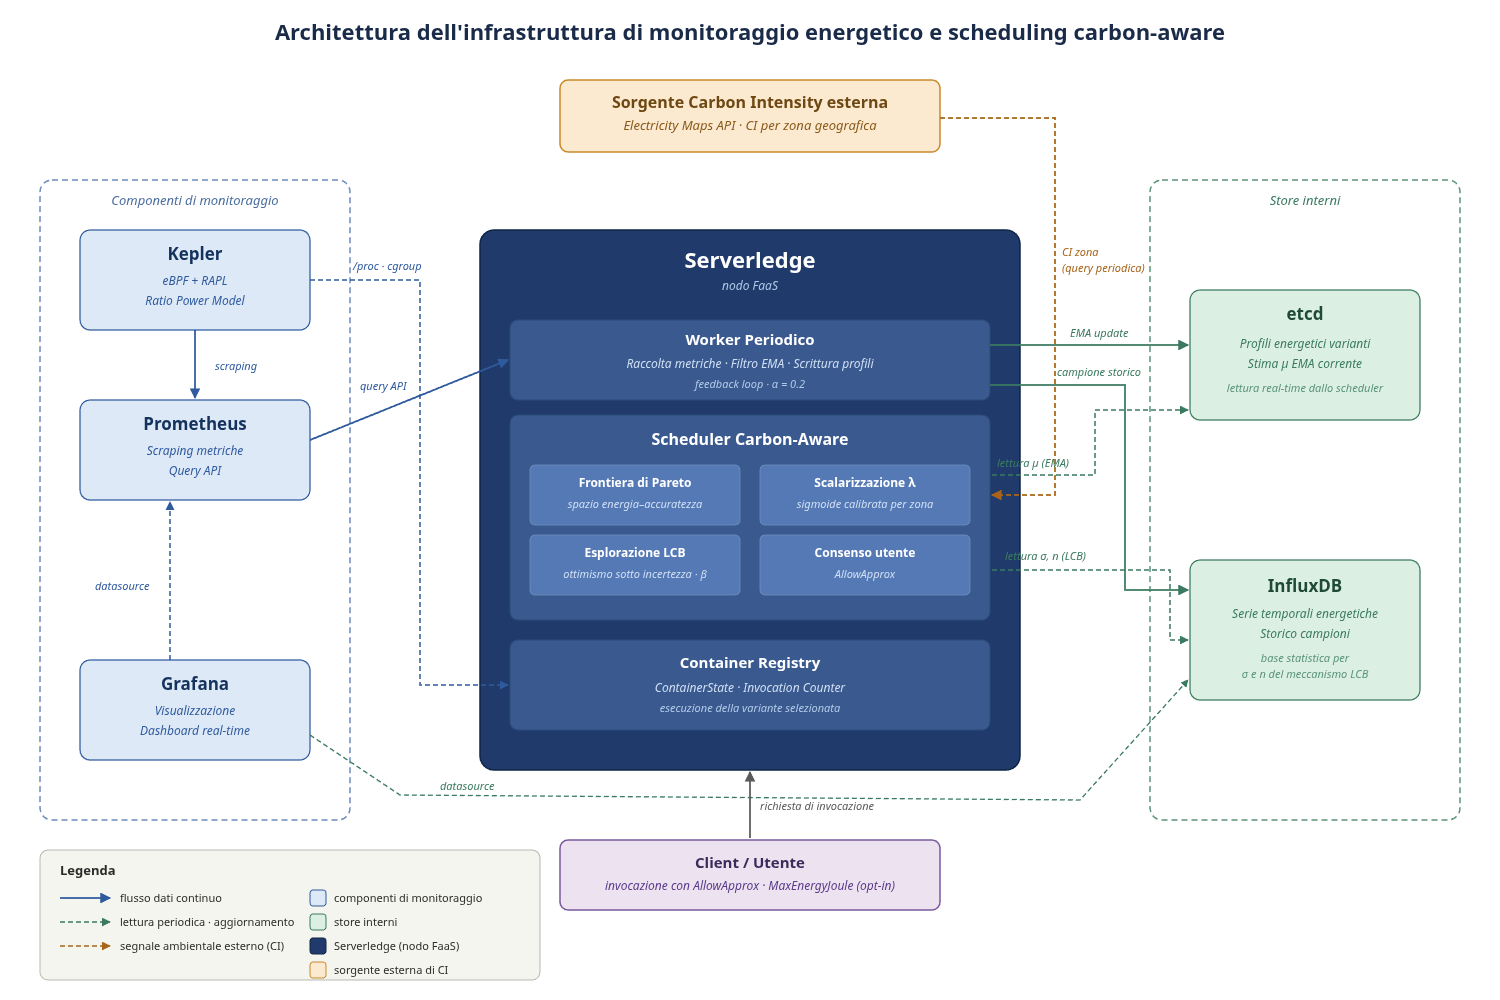
\includegraphics[width=0.85\textwidth]{figures/infrastracture-diagram.png}
    \caption{Architettura dell'infrastruttura di monitoraggio energetico e scheduling
carbon-aware. I componenti di monitoraggio esterni (Kepler, Prometheus, Grafana)
sono separati dagli store interni (etcd, InfluxDB), con Serverledge al centro
che interagisce con entrambi i livelli. Lo scheduler carbon-aware integra la
logica di selezione della variante — basata su frontiera di Pareto, scalarizzazione
tramite $\lambda$, esplorazione LCB e consenso utente — e riceve il segnale di
carbon intensity tramite query periodica a una sorgente esterna.}
    \label{fig:infra-arch}
\end{figure}

I componenti avviati,  come mostrato anche in Figura~\ref{fig:infra-arch}, sono i seguenti:

\begin{itemize}
    \item \textbf{Kepler}: eseguito in modalità privilegiata con accesso
 a \texttt{/sys}, \texttt{/proc} e al socket Docker dell'host, 
    condizioni necessarie per la lettura dei contatori RAPL e 
    l'associazione dei consumi ai container tramite cgroup.
    
    \item \textbf{Prometheus}: configurato per effettuare lo scraping 
    periodico delle metriche esposte da Kepler, rendendole disponibili 
    tramite API di interrogazione.
    
    \item \textbf{InfluxDB}: database a serie temporali utilizzato per 
    l'archiviazione storica dei campioni energetici prodotti dal 
    sistema ad ogni ciclo di raccolta.
    
    \item \textbf{etcd}: store distribuito chiave-valore che funge da 
    registro delle funzioni e delle relative varianti, inclusi i profili 
    energetici aggiornati dinamicamente a runtime.
    
    \item \textbf{Grafana}: strumento di visualizzazione utilizzato per 
    il monitoraggio in tempo reale dei consumi durante gli esperimenti.
\end{itemize}

Una volta avviata, l'infrastruttura opera in modo autonomo: Kepler 
rileva i container Docker presenti sull'host e ne aggiorna le metriche 
energetiche ad ogni ciclo di campionamento; Prometheus le raccoglie e 
le rende interrogabili; il sistema interno di Serverledge, descritto nelle sezioni successive,
le legge periodicamente --- limitatamente ai container attivi da esso gestiti --- per aggiornare i profili energetici 
delle varianti di funzione. Il segnale di carbon intensity, necessario allo scheduler 
per la selezione carbon-aware della variante, non è parte di questa infrastruttura: 
viene acquisito dallo scheduler a runtime tramite query periodica a una 
sorgente esterna, come descritto nella Sezione~\ref{cap:scheduler}.